%%%%%%%%%%%%%%%%%%%%%%%%%%%%%%%%%%%%%%%%%
% Arsclassica Article
% LaTeX Template
% Version 1.1 (10/6/14)
%
% This template has been downloaded from:
% http://www.LaTeXTemplates.com
%
% Original author:
% Lorenzo Pantieri (http://www.lorenzopantieri.net) with extensive
% modifications by:
% Vel (vel@latextemplates.com)
%
% License:
% CC BY-NC-SA 3.0 (http://creativecommons.org/licenses/by-nc-sa/3.0/)
%
%%%%%%%%%%%%%%%%%%%%%%%%%%%%%%%%%%%%%%%%%

%-------------------------------------------------------------------------------
%	PACKAGES AND OTHER DOCUMENT CONFIGURATIONS
%-------------------------------------------------------------------------------

\documentclass[
10pt, % Main document font size
a4paper, % Paper type, use 'letterpaper' for US Letter paper
oneside, % One page layout (no page indentation)
%twoside, % Two page layout (page indentation for binding and different headers)
headinclude,footinclude, % Extra spacing for the header and footer
BCOR5mm, % Binding correction
]{scrartcl}

%%%%%%%%%%%%%%%%%%%%%%%%%%%%%%%%%%%%%%%%%
% Arsclassica Article
% Structure Specification File
%
% This file has been downloaded from:
% http://www.LaTeXTemplates.com
%
% Original author:
% Lorenzo Pantieri (http://www.lorenzopantieri.net) with extensive modifications by:
% Vel (vel@latextemplates.com)
%
% License:
% CC BY-NC-SA 3.0 (http://creativecommons.org/licenses/by-nc-sa/3.0/)
%
%%%%%%%%%%%%%%%%%%%%%%%%%%%%%%%%%%%%%%%%%

%----------------------------------------------------------------------------------------
%	REQUIRED PACKAGES
%----------------------------------------------------------------------------------------

\usepackage[
nochapters, % Turn off chapters since this is an article        
beramono, % Use the Bera Mono font for monospaced text (\texttt)
eulermath,% Use the Euler font for mathematics
pdfspacing, % Makes use of pdftex’ letter spacing capabilities via the microtype package
dottedtoc % Dotted lines leading to the page numbers in the table of contents
]{classicthesis} % The layout is based on the Classic Thesis style

\usepackage{arsclassica} % Modifies the Classic Thesis package

\usepackage{fontenc} % Use 8-bit encoding that has 256 glyphs

\usepackage[utf8]{inputenc} % Required for including letters with accents

\usepackage{graphicx} % Required for including images
\graphicspath{{Figures/}} % Set the default folder for images

\usepackage{enumitem} % Required for manipulating the whitespace between and within lists


\usepackage{subfig} % Required for creating figures with multiple parts (subfigures)

\usepackage{amsmath,amssymb,amsthm} % For including math equations, theorems, symbols, etc

\usepackage{algorithm}
\usepackage{algpseudocode}

\usepackage[numbered,framed]{matlab-prettifier}

\usepackage[numbers]{natbib}

\usepackage{geometry}
\geometry{lmargin=1.1in, bmargin=0.9in, tmargin=0.9in, rmargin=1.1in}

%----------------------------------------------------------------------------------------
%	THEOREM STYLES
%---------------------------------------------------------------------------------------

\theoremstyle{definition} % Define theorem styles here based on the definition style (used for definitions and examples)
\newtheorem{definition}{Definition}

\theoremstyle{plain} % Define theorem styles here based on the plain style (used for theorems, lemmas, propositions)
\newtheorem{theorem}{Theorem}

\theoremstyle{remark} % Define theorem styles here based on the remark style (used for remarks and notes)

%----------------------------------------------------------------------------------------
%	HYPERLINKS
%---------------------------------------------------------------------------------------

\hypersetup{
%draft, % Uncomment to remove all links (useful for printing in black and white)
colorlinks=true, breaklinks=true, bookmarks=true,bookmarksnumbered,
urlcolor=RoyalBlue, linkcolor=RoyalBlue, citecolor=webgreen, % Link colors
pdftitle={}, % PDF title
pdfauthor={Nouce}, % PDF Author
pdfsubject={Optimization}, % PDF Subject
pdfkeywords={}, % PDF Keywords
pdfcreator={pdfLaTeX}, % PDF Creator
pdfproducer={LaTeX with hyperref and ClassicThesis} % PDF producer
}


\input{/home/york/Document/reading/latex/definedsymbol.tex}

% Specify custom hyphenation points in words with dashes where you would like 
% hyphenation to occur, or alternatively, don't put any dashes in a word to 
% stop hyphenation altogether
\hyphenation{Fortran hy-phen-ation} 

%-------------------------------------------------------------------------------
%	TITLE AND AUTHOR(S)
%-------------------------------------------------------------------------------

\title{\normalfont\spacedallcaps{Optimizing Composite Functions}} 

% The article author(s) - author affiliations need to be specified in the 
% AUTHOR AFFILIATIONS block
\author{\spacedlowsmallcaps{A *} \\ 
\texttt{\href{mailto:A@gmail.com}{A@gmail.com}} }

\date{\today} % An optional date to appear under the author(s)

%-------------------------------------------------------------------------------

\newcommand{\Sgprox}{\mathbf{gprox}}

\begin{document}

%-------------------------------------------------------------------------------
%	HEADERS
%-------------------------------------------------------------------------------

\renewcommand{\sectionmark}[1]{\markright{\spacedlowsmallcaps{#1}}} 
% The header for all pages (oneside) or for even pages (twoside)
% \renewcommand{\subsectionmark}[1]{\markright{\thesubsection~#1}} 
% Uncomment when using the twoside option - this modifies the header on odd 
% pages
\lehead{\mbox{\llap{\small\thepage\kern1em\color{halfgray} 
\vline}\color{halfgray}\hspace{0.5em}\rightmark\hfil}} % The header style

\pagestyle{scrheadings} % Enable the headers specified in this block

%-----------------------------------------------------------------------------
%	TABLE OF CONTENTS & LISTS OF FIGURES AND TABLES
%-----------------------------------------------------------------------------

\maketitle % Print the title/author/date block

% Set the depth of the table of contents to show 
% sections and subsections only
\setcounter{tocdepth}{2} 

\tableofcontents % Print the table of contents

\listoffigures % Print the list of figures

\listoftables % Print the list of tables

%------------------------------------------------------------------------------
%	ABSTRACT
%------------------------------------------------------------------------------

\section*{Abstract} 
% This section will not appear in the table of contents due to the star 
% (\section*)

% \lipsum[1] % Dummy text
Many problems of relevance in bioinformatics, signal processing, and statistical 
learning can be formulated as minimizing a composite function: a smooth 
function and  non-smooth function. There are some generic methods that could be 
used to solve this optimization problem theoretically, such as CVX, FISTA, ADMM 
and PNOPT. In addition, the stochastic methods including SGD and stochastic 
ADMM are well suited to handle large data sets. We will introduce these methods 
one by one, and analyze their strengths and weaknesses through the numerical 
experiments.



%-------------------------------------------------------------------------------
%	AUTHOR AFFILIATIONS
%-------------------------------------------------------------------------------

{\let\thefootnote\relax\footnotetext{* \textit{Department of Computer Sciences, 
SJTU}}}


%-------------------------------------------------------------------------------

\newpage 
% Start the article content on the second page, remove this if you have a longer 
% abstract that goes onto the second page

%-------------------------------------------------------------------------------
%	INTRODUCTION
%-------------------------------------------------------------------------------

\section{Introduction}
\paragraph{}
In this survey, we are concerned with the following optimization problem: 
\begin{equation} \label{eq:main_problem}
	\min_{\Vx \in \SetR^p} \CompF{\Vx} \triangleq g(\Vx) + \Psi(\Vx),
\end{equation}
where $ g $ is a convex and continuously differentiable loss function, and 
$\Psi $ is usually defined as a (non-smooth) convex penalty function or 
regularizer. For example, $\Psi(\Vx) \triangleq \lambda_1 \norm{\Vx}_2 $ 
is a ridge regression , and  $\Psi(\Vx) \triangleq \lambda_1 \norm{\Vx}_1 $ 
defines a LASSO penalty \cite{tibshirani1996regression}.

Indeed, there are plenty of machine learning models, which  can be cast into 
this formulation in (\ref{eq:main_problem}), such as the generalized lasso 
\cite{tibshirani2011solution}, the group lasso for logistic regression 
\cite{meier2008group}. Moreover, many real-world problems benefit from 
these models such as Gene expression and time-varying network. In this paper we 
mainly study computational issue  of the model in (\ref{eq:main_problem}).

There are a variety of methods to solve these models, such as SpaRSA 
\cite{wright2009sparse} and LARS \cite{efron2004least}.
We focus on the generic methods:
% [noitemsep] removes whitespace between the items for a compact look
\begin{enumerate}[noitemsep] 
	\item CVX. 
	We can use CVX \cite{cvx} to conveniently formulate and solve many 
complex convex programs. Constraints and objectives that are expressed using 
these rules are automatically transformed to a canonical form and solved.
% 	We can use CVX \cite{cvx} to conveniently formulate and solve 
% constrained norm minimization, entropy maximization, determinant 
% maximization, 
% and many other complex convex programs. Constraints and objectives that are 
% expressed using these rules are automatically transformed to a canonical form 
% and solved. CVX \textbf{will} solve many medium and large scale problems, 
% provided they have exploitable structure (such as sparsity).

	\item Proximal Gradient Descent. The base operation of proximal methods is 
evaluating the proximal operator of a function. There are a large number of 
examples of proximal operators that commonly arise in practice like LASSO and 
elastic net. 
%	Proximal methods \cite{parikh2013proximal} 
%sit at a higher level of abstraction than classical algorithms like Newton's 
%method: the base operation is evaluating the proximal operator of a function, 
%which itself involves solving a small convex optimization problem. These 
%subproblems, which generalize the problem of projecting a point onto a convex 
%set, often admit closed-form solutions or can be solved very quickly with 
%standard or simple specialized methods. There are a large number of examples 
%of 
%proximal operators that commonly arise in practice like LASSO and elastic net. 
%\citet{nesterov1983method} proposed a scheme to accelerate first-order methods,
%this scheme could be applied to non-smooth case by using proximal gradient 
%descent as shown in FISTA \cite{beck2009fast} and N07 
%\cite{nesterov2007gradient}.

	\item ADMM. 
	The alternating direction method of multipliers (ADMM) 
\cite{boyd2011distributed} is very similar to proximal methods but more 
general, and ADMM is well suited to distributed convex optimization.

% and in particular to large-scale problems arising in statistics, machine 
% learning, and related areas. The ADMM method could by applied to a wide 
% variety 
% of statistical and machine learning problems of recent interest, including 
% the 
% lasso, sparse logistic regression, basis pursuit, covariance selection, 
% support vector machines, and many others. 

	\item Newton-type methods. The main idea is to approximate the smooth part 
of the objective function using the second order information. Then the 
computation is shift to solve the subproblem.
	

	\item Coordinate Descent. When the objective is separable, we could 
Optimize the model according to each coordinate.
	

	\item SGD. In stochastic gradient descent, the true gradient is approximated 
by a gradient at a single example. SGD is very efficient to obtain a less 
accuracy solutions. 
	

\end{enumerate}

We will introduce these methods one by one, and analyze their strengths and 
weaknesses through the numerical experiments.


%---------------------------------------------------------------------------
%	Illustration and Numerical Experiments
%---------------------------------------------------------------------------

\section{Illustrations}
\paragraph{}
In this section, we illustrate the basic concept of these methods in detail.
To understand these methods more thoroughly, we give some comparative 
experiments.



%------------------------------------------------

\subsection{CVX}
\subsubsection{Basic Concept}
\paragraph{}
CVX is a Matlab-based modeling system for convex 
optimization. The convex optimization problems is constructed by 
\textit{disciplined convex 	programming}. The default solver is currently SDPT3 
\cite{toh1999sdpt3} which is designed to solve conic programming problems whose 
constraint cone is a product of semidefinite cones, second-order cones, and/or 
non-negative orthants. It employs a predictor-corrector primal-dual 
path-following method, with either the HKM or the NT search direction.
CVX utilizes symmetric primal/dual solvers that simply cannot support the 
functions from the exponential family natively. CVX constructed a successive 
approximation heuristic that allows the symmetric primal/dual solvers to support 
the exponential family of functions. However, it will sometimes fail to 
converge even for problems known to have solutions. Even when it does converge, 
it is several times slower than the standard solver, due to its iterative 
approach.

\subsubsection{Matlab Implementation}
\paragraph{}
CVX turns Matlab into a modeling language, allowing constraints 
and objectives to be specified using standard Matlab expression syntax.
For example, consider the following convex optimization model (LASSO):
\begin{align}
	min~& \norm{ \MA \Vx - \Vb }_2 	\nonumber \\
	s.t.~& \norm{ \Vx }_1 \leq d.  \nonumber 
\end{align}
or equivalent,
\begin{align} \label{eq:lasso_formulation}
	min~& \frac{1}{2} \norm{ \MA \Vx - \Vb }_2^2 + \lambda \norm{ \Vx }_1 
\end{align}
We can use CVX to solve this model via the following matlab code:

\begin{lstlisting}[
  style=Matlab-editor,
  basicstyle=\mlttfamily\small,
  escapechar=`,
  caption = {Solve LASSO using CVX}
  ]
cvx`\_`begin
  variable x(n)
  minimize(norm(A * x - b, 2))
  subject to
    norm(x, 1) `$<$`= d
cvx`\_end``
\end{lstlisting}


CVX will solve many medium and large scale problems, provided they have 
exploitable structure (such as sparsity), eliminated for loops and functions 
like $log$ and $exp$ that require successive approximation. We test the 
performance of CVX in several datasets, the Matlab code is located in 
folder \textit{matlab/cvx\_test}.




\subsection{Proximal Gradient Descent} \label{sec:proximal_algorithm}
\subsubsection{Basic Concept} 
\paragraph{}
Proximal algorithms can be viewed as a standard 
tool for non-smooth, constrained, large-scale, or distributed problems. They 
are very generally applicable, but they turn out to be especially well-suited 
to problems of recent and widespread interest involving large or 
high-dimensional datasets. The base operation of proximal algorithms is 
evaluating the proximal operator of a function, which involves solving a small 
convex optimization problem. These subproblems can be solved with standard 
methods, but they often admit closed form solutions or can be solved very 
quickly with simple specialized methods.  

The proximal operator $\Sprox_{\lambda f}: \SetR^n \to \SetR^n $ of 
the scaled function $ \lambda f $, where $ \lambda > 0 $ , is defined by 
\begin{equation} \label{eq:proximal_operator_definition}
	\Sprox_{\lambda f}(v) = \Sargmin{x}
	\left( f(x) + \frac{1}{2\lambda}\norm{x - v}_2^2 \right).
\end{equation}
There are various interpretations of the proximal operator illustrated in 
\cite{parikh2013proximal}. 

We could evaluate the proximal operator \eqref{eq:proximal_operator_definition} 
using iterative methods such as gradient methods and L-BFGS when $f$ is smooth. 
If the minimization is over a convex constrained set, we can use CVX to obtain 
the proximal operator. A fully separable function $f$ reduces to evaluating the 
proximal operator of a scalar convex function. For a non-smooth example, if 
$f(x) = \abs{x}$, then we have that
\begin{align} \label{eq:soft_thresholding}
	S_{\lambda}(v) = \Sprox_{\lambda f}(v) = 
	\begin{cases} 
		v - \lambda, & v > \lambda \\ 
		0,		    & \abs{v} \leq \lambda \\ 
		v + \lambda, & v < -\lambda,
	\end{cases} 
\end{align}
which is called \textit{soft thresholding}.

From the the Moreau envelope perspective, that Moreau envelope or Moreau-Yosida 
regularization $M_{\lambda f}$ of the function $\lambda f$ is define as,
\begin{equation*}
	M_{\lambda f}(v) = \inf_{x} \left( f(x) + 
	\frac{1}{2\lambda} \norm{x-v}_2^2  \right).
\end{equation*}
The Moreau envelope $M_f$ is essentially a smoothed or regularized
form of $f$: It has domain $\SetR^n$, even when $f$ does not, and it is 
continuously differentiable, even when $f$ is not. In addition, the sets of 
minimizers of $f$ and $M_f$ are the same. The problems of minimizing 
$f$ and $M_{f}$ are thus equivalent, and the latter is always a smooth 
optimization problem. Because $M_f^{**} = M_f $ and the infimal convolution is 
dual to addition, it follows that
\begin{align}
	M_f &= ((M_f)^*)^* \nonumber\\
	    &= (f^* +  \frac{1}{2} \norm{\cdot}_2^2)^*.
\end{align}
In general, the conjugate $\phi^*$ of a closed proper convex function $\phi$ is 
smooth when $\phi$ is strongly convex. This suggests that the Moreau envelope 
$M_f$ can be interpreted as obtaining a smooth approximation to a function by 
taking its conjugate, adding regularization, and then taking the conjugate 
again.

From Eqn. \eqref{eq:proximal_operator_definition}, we know that proximal 
minimizing is smooth the primal objective. For example, applying this technique 
to $ \abs{x} $, gives the Huber function.
\begin{equation*}
	(\abs{x}^* + \frac{1}{2} \norm{x}_2^2)^* = \phi^{\text{huber}}(x)
\end{equation*}


This perspective is very related to 
recent work by Nesterov\cite{nesterov2005smooth}. Then minimize the 
non-smooth objective is equivalent to minimize the smoothed objective $M_f$.

There is a wide literature on applying various 
proximal algorithms to particular problems or problem domains, we describe
the proximal minimization algorithm and proximal gradient method respectively.

\subsubsection{Proximal Minimizing Algorithm}
\paragraph{}
The proximal minimization algorithm, also called proximal iteration or the 
proximal point algorithm, is 
\begin{equation} \label{eq:proximal_min_subproblem}
	x^{k+1} = \Sprox_{\lambda f} (x^k),
\end{equation}
where $ f $ is a closed proper convex function, and $x^k$ denotes the $k$th 
iterate of the algorithm. If $f$ has a minimum, then $x^k$ converges to the set 
of minimizers of $f$ and $f(x^k)$ converges to its optimal value 
\cite{bauschke2011convex}. A simple interpretation is as disappearing Tikhonov 
regularization, that the quadratic (Tikhonov) regularization 'goes away' 
in the limit. Moreover, the proximal operator of the second-order 
approximation can be viewed as the trust-region method with a 
Levenberg-Marquardt update, that
\begin{align} \label{eq:quadratic_proximal_minimizing}
	& \Sprox_{\lambda \hat{f}_v} (v) = 
	v - (\nabla^2 f(v) + \frac{1}{\lambda}\MI)^{-1}\nabla f(v), \\
\text{where~} & \hat{f}_v = f(v) + \nabla f(v)^T (x - v) +
	\frac{1}{2} (x-v)^T \nabla^2 f(v) (x - v). \nonumber
\end{align}

The (sub)problem \eqref{eq:proximal_min_subproblem} 
becomes easier for gradient method as more quadratic regularization is added. 
Here, 'easier' can mean fewer iterations, faster convergence, or higher 
reliability. The proximal algorithm would be useful in a situation where it is 
hard to minimize the function $f$ (our goal), but easy (or at least easier) to 
minimize $f$ plus a quadratic like iterative refinement for solving linear 
equations. Besides, it will play an important role in solving ill-conditioned 
smooth minimization problems.

\subsubsection{Proximal Gradient Method}
\paragraph{}
Consider the problem \eqref{eq:main_problem}, where $g:  \SetR^n \to \SetR $ and 
$\Psi: \SetR^n \to \SetR \cup {+\infty}$ are 
closed proper convex and $g$ is differentiable. In this form, we split the 
objective into two terms, one of which is differentiable. The proximal gradient 
method is
\begin{align} \label{eq:proximal_gradient_descent}
	\Vx^{k+1} = \Sprox_{\lambda^k \Psi}(\Vx^k - \lambda^k \nabla g(\Vx^k)), 
\end{align}
where $ \lambda^k > 0 $ is a step size. The proximal gradient can be interpreted 
as majorization-minimization algorithm or fixed point iteration 
\cite{parikh2013proximal}.  This method can be shown to converge with rate 
$ \CompO{ \frac{1}{k} } $, and the accelerated version \cite{beck2009fast} 
(optimal first-order method) converges with rate $ \CompO{ \frac{1}{k^2} } $. 
We could solve LASSO problem \eqref{eq:lasso_formulation} directly using 
Eqn. \eqref{eq:soft_thresholding} and \eqref{eq:proximal_gradient_descent}. 
There is an excellent software package called TFOCS \cite{becker2012tfocs} is 
based on and contains several implementations of such accelerated proximal 
gradient methods. One of these accelerated proximal gradient methods 
(N07\cite{nesterov2007gradient}) is described in Algorithm 
\ref{alg:lasso_proximal_solver}, the proximal operator of $ \Psi $ should be 
easy to evaluate. There are several ways to estimate $L$ as discussed in 
\cite{becker2012tfocs}.

\begin{algorithm}[ht]
	\caption{Solve composite functions \eqref{eq:main_problem} via proximal 
gradient method}
\label{alg:lasso_proximal_solver}
\begin{algorithmic}[1]
	\Require $ \Vz^0 \in \SetR^n $, Lipschitz estimate $ L $
	\State $\theta^0 \gets 1, \Vv^0 \gets \Vz^0, j \gets 0 $
	\Repeat
	\State $ \Vy^j\gets 
	(1-\theta^j)\Vz^j + \theta^j \Vv^j $
	\State {\small $ \Vv^{j+1} \gets 
	\Sargmin{\Vz} \langle 
	(\theta^j)^2 \sum_{i=0}^j (\theta^i)^{\minus 1} \nabla g(\Vy^i) , \Vz
	\rangle  + \frac{1}{2} (\theta^j)^2 L \norm{ \Vz - \Vz_0 }^2 + \Psi(\Vz) $}
	\State  $ \Vz^{j+1} \gets \Sargmin{\Vz} \langle \nabla g(\Vy^j), z \rangle 
	+ \frac{1}{2} L \norm{ \Vz - \Vy^j }^2 + \Psi(\Vz) $
	\State $ \theta^{j+1} \gets 2/(1+(1+4/(\theta^{j})^2)^{\frac{1}{2}})$
	\State $ j \gets j + 1 $
\Until{some stopping condition is satisfied}
\end{algorithmic}
\end{algorithm}

\subsubsection{Dual Approach}
\paragraph{}
Unlike \citet{nesterov2005smooth}'s approach which applied the smoothing 
technique to the primal objective, we consider the dual approach presented in 
TFOCS\cite{becker2012tfocs}. The dual approach smooth the dual objective, 
specifically, 
\begin{align*}
	M_g(\Vv) &= \inf_{\Vx} (g(\Vx) + \frac{1}{2}\norm{\Vx-\Vv}_2^2) \nonumber \\
	&= (g(\Vx)^* + \frac{1}{2}\norm{\Vx-\Vv}_2^2)^* \nonumber \\
	&= (f(\Vx) + \frac{1}{2}\norm{\Vx-\Vv}_2^2)^*. \nonumber
\end{align*}
Minimizing $f(\Vx) + \frac{1}{2} \norm{\Vx-\Vx_0}_2^2 $ is equivalent to 
maximizing the dual $M_g(\Vv)$. There is a more general model called smoothed 
conic dual (SCD) model introduced in TFOCS \cite{becker2012tfocs} which could 
solve the more general non-smooth models like the fused LASSO.  It's easy to 
show that the gradient of the dual is Lipschitz continuous if the primal is 
strongly convex\cite{nesterov2005smooth}, then provably convergent, accelerated 
gradient methods in the Nesterov style are possible.

Consider the statistical model that $\Psi(\Vx) = \norm{\MF \Vx}_1 $ in Eqn. 
\eqref{eq:main_problem}, we could solve this model via SCD as shown 
in Algorithm \ref{alg:scd_solver}. However, it does not solve the problem 
exactly because the proximal function $ \frac{\rho}{2} \norm{\Vx-\Vx_0}_2^2 $, 
by applying proximal iteration \eqref{eq:proximal_min_subproblem} (which 
called continuation in TFOCS), we could obtain the exact solutions. The main 
burden of Algorithm \ref{alg:scd_solver} is line \ref{ln:main_burden} which may 
be inefficient to find the minimizer.

\begin{algorithm}[ht]
\caption{Solve Composite Function via SCD}\label{alg:scd_solver}
\begin{algorithmic}[1]
	\Require $ \Vz^0, \Vx^0, \rho > 0 $
	\State $ \theta^0 \gets 1, \Vv^0 \gets \Vz^0, j \gets 0 $
\Repeat
	\State $ \Vy^j \gets (1-\theta^j)\Vv^j + \theta^j \Vz^j $
	\State \label{ln:main_burden}
	$\hat{\Vx} \gets \Sargmin{\Vx} g(\Vx) + \frac{\rho}{2} \norm{\Vx-\Vx_0}_2^2
	- \Vx^T \MF^T\Vy^j $ 
	\State  $ \Vz^{j+1} \gets \Sargmin{\Vz: \norm{\Vz}_{\infty} \leq 1} 
	\frac{\theta^j}{2\delta^j}\|\Vz-\Vz^j\|_2^2 + \Vz^T \MF\hat{\Vx}  $
	\State  $ \Vv^{j+1} \gets (1-\theta^j)\Vv^j + \theta^j \Vz^{j+1}  $
 \State $ \theta^{j+1} \gets 2/(1+(1+4/(\theta^j)^2)^{\frac{1}{2}}) $
 \State $ j \gets j + 1 $
\Until{some stopping condition is satisfied}
\end{algorithmic}
\end{algorithm}


\subsection{ADMM}
\subsubsection{Basic Concept}
\paragraph{}
ADMM was first introduced in the mid-1970s by Gabay, Mercier, Glowinski, and 
Marrocco, though similar ideas emerged as early as the mid-1950s. It turns out 
to be equivalent or closely related to many other algorithms as well, such as 
Douglas-Rachford splitting from numerical analysis, Spingarn's method of partial 
inverses, Dykstra's alternating projections method, Bregman iterative algorithms 
for $\ell_1$ problems in signal processing, proximal methods, and many others.

ADMM is an algorithm that is intended to blend the decomposability of dual 
ascent with the superior convergence properties of the method of multipliers. 
The algorithm solves problems in the form
\begin{equation}
	\begin{split}
    \min~& g(\Vx) + \Psi(\Vz) \\
	s.t.~& \MA \Vx + \MB \Vz = \Vc,
	\end{split}
\end{equation}
with $\Vx \in \SetR^n$ and $z \in \SetR^m$, where $ \MA \in \SetR^{p \times n} 
$, $\MB \in \SetR^{p \times m}$, and $c \in \SetR^p$. Assuming that $f$ and $g$ 
are convex, we form the augmented Lagrangian 
\begin{equation*}
L_\rho(\Vx, \Vz, \Vy) = g(\Vx) + \Psi(\Vz) + \Vy^T(\MA\Vx + \MB \Vz - \Vc) + 
\frac{\rho}{2} \norm{\MA\Vx + \MB\Vz - \Vc}_2^2.
\end{equation*}
ADMM consists of the iterations
\begin{align}
	\Vx^{k+1}& \gets \Sargmin{\Vx} L_\rho(\Vx, \Vz^k, \Vy^k) \nonumber \\
	\Vz^{k+1}& \gets \Sargmin{\Vz} L_\rho(\Vx^{k+1}, \Vz, \Vy^k) \nonumber \\
	\Vy^{k+1}& \gets \Vy^k + \rho (\MA \Vx^{k+1} + \MB \Vz^{k+1} - \Vc), 
\nonumber
\end{align}
where $\rho > 0$. The algorithm is very similar to dual ascent and the method of 
multipliers where the augmented Lagrangian is minimized jointly with respect to 
the two primal variables. In ADMM, on the other hand, $\Vx$ and $\Vz$ are 
updated in an alternating or sequential fashion, which accounts for the term 
alternating direction. \citet{boyd2011distributed} explained the ADMM in 
detail.

There are many convergence results for ADMM discussed in the 
literature, under some assumptions, ADMM converges linearly 
\cite{nishihara2015general}. However simple examples show that ADMM can be very 
slow to converge to high accuracy. Fortunately, it is often the case that ADMM 
converges to modest accuracy within a few tens of iterations which is sufficient 
for many applications. 

\subsubsection{Proximal Operator In ADMM}
\paragraph{}
Consider the simple case where $\MA = \MI$, which appears frequently. Then the 
$\Vx$-update issue
\begin{equation*}
	\Vx^{+} = \Sargmin{\Vx}  f(\Vx) + \frac{\rho}{2} \norm{\Vx - \Vv}_2^2,
\end{equation*}
which is exactly the proximal operator as 
\eqref{eq:proximal_operator_definition}. The same method discussed 
in Section \ref{sec:proximal_algorithm} could be applied to evaluating 
the update of ADMM. For instance, if $ f(\Vx) = \abs{\Vx} $, then the 
$\Vx$-update could be calculated by $S_{1 / \rho}(\Vv)$ as shown in 
Eqn. \eqref{eq:soft_thresholding}.

\subsubsection{Generalized LASSO}
\paragraph{}
The lasso problem can be generalized to
\begin{equation} \label{eq:fused_lasso}
	\min \frac{1}{2}\norm{\MA \Vx - \Vb}_2^2 + \lambda \norm{\MF \Vx}_1
\end{equation}
where $\MF$ is an arbitrary linear transformation. An important special case is 
fused LASSO when $\MF \in \SetR^{(n-1) \times n}$ is the difference matrix,
\begin{equation*}
\MF_{ij} =  
	\begin{cases} 1 &\mbox{if }  i = j \\
	\minus{1} & \mbox{if } j = i+1 \\
	0 & otherwise.\end{cases} 
\end{equation*}
In ADMM form, the problem \eqref{eq:fused_lasso} can be written as
\begin{align}
	\min~& \frac{1}{2}\norm{\MA \Vx - \Vb}_2^2 + \lambda \norm{\Vz}_1
	\nonumber \\
	s.t.~& \MF\Vx - \Vz = 0, \nonumber
\end{align}
which yields the ADMM iteration in Algorithm \ref{alg:admm_fusedlasso}.
\begin{algorithm}[ht]
\caption{ADMM for Fused LASSO}\label{alg:admm_fusedlasso}
\begin{algorithmic}[1]
\Require $ \Vz_0$ and $\Vu_0$
\State $ k \gets 0 $
\Repeat
\State $\Vx^{k+1} \gets (\MA^T\MA + \rho \MF^T \MF)^{\minus{1}} (\MA^T\Vb + 
\rho \MF^T(\Vz^k - \Vu^k)) $
\State $\Vz^{k+1} \gets S_{\frac{\lambda}{\rho}}(\MF\Vx^{k+1} + \Vu^k) $
\State $\Vu^{k+1} \gets \Vu^k + \MF \Vx^{k+1} - \Vz^{k+1}$
\State $k \gets k+1$
\Until{stopping condition is satisfied}
\end{algorithmic}
\end{algorithm}


It easy to see that ADMM is much powerful than proximal algorithm. Besides, 
ADMM is readily to do distributed optimization via global variable consensus 
\cite{boyd2011distributed}.


\subsection{Newton-type Methods}
\subsubsection{Basic Concept}
\paragraph{}


In order to solve the problem more precisely in modest time, we resort to 
Newton approach which use the second information. More specifically, we use 
information from the second derivative to form a quadratic approximation to a 
function like \eqref{eq:quadratic_proximal_minimizing}. Consider the problem 
\eqref{eq:main_problem}, we appropriate the smooth part $g$, which results
\begin{align} \label{eq:proximal_local_model_expend}
	\hat{\mathcal{F}} (\Vx) &= \hat{g}(\Vx) + \Psi(\Vx) =  g(\Vx_k) + \nabla 
	g(\Vx_k)^T (\Vx - \Vx_k) + \frac{1}{2}(\Vx-\Vx_k)^T \MH_k (\Vx - \Vx_k) 
	+ \Psi(\Vx),
\end{align}
where $ \MH_k $ is a $p\times p$ (semi)definite positive matrix as 
approximation 
to the  Hessian of $ g$ at $\Vx=\Vx_k$. There are many strategies for choosing 
$ \MH_k $, such as BFGS and LBFGS \cite{nocedal2006numerical}. 
There has been a flurry of activity about developments of Newton-type methods 
for minimizing composite functions in the literature. In particular, 
\citet{lee2014proximal} focused on minimizing a composite function, which 
contains a convex smooth function and a convex non-smooth function with a 
simple proximal mapping. They also analyzed the convergence rate of various 
proximal Newton-type methods. 
\citet{schmidt2009optimizing,schmidt2011projected} discussed a projected 
quasi-Newton algorithm, but the sub-iteration costs too much.


Compare to the 
proximal operator \eqref{eq:proximal_operator_definition}, Eqn. 
\eqref{eq:proximal_local_model_expend} could be expressed as the generalized 
proximal operator
\begin{equation*} \label{eq:generalized_proximal_operator}
	\Sgprox_{\MH \Psi}(\Vv) = \Sargmin{\Vx}
	\left( \Psi(\Vx) + \frac{1}{2}(\Vx-\Vv)^T \MH (\Vx - \Vv) \right).
\end{equation*}
Usually, $\Sgprox$ is not as easy as $\Sprox$ operator to calculate.
It would be equivalent to $\Sprox$ operator when $ \MH $ is a diagonal matrix, 
and there's an straightforward method called spectral projected gradient (SPG) 
\cite{birgin2000nonmonotone} adopted this strategy. There also have some more 
complex and efficient ways like the ``diagonal+rank-1 case'' studied by 
\citet{becker2012quasi}. Here we focus on the most general case when $ \MH $ is 
approximated via BFGS, which proved to converge superlinearly 
\cite{lee2014proximal}.

\subsubsection{Proximal Newton-type Method}
\paragraph{}
Though it is not straightforward to solve the subproblem 
\eqref{eq:proximal_local_model_expend}, we could apply the iterative method. 
Obviously, \eqref{eq:proximal_local_model_expend} is a quadratic problem which 
could be solved via CVX, FISTA, ADMM and SPG. We have found that FISTA performs 
best empirically. Given Algorithm \ref{alg:lasso_proximal_solver}, we only need 
to obtain $\nabla g(\Vx)$, and 
$ \nabla g(\Vx) = \nabla g(\Vx_k) + \MH_k(\Vx - \Vx_k) $ 
in this subproblem, so the LBFGS is appreciate and we could solve this 
subproblem with $\CompO{\frac{1}{k^2}} $ complexity. The whole proximal 
quasi-Newton method is illustrated in Algorithm \ref{alg:PQN}.

\begin{algorithm}[ht]
\caption{The proximal quasi-Newton method}\label{alg:PQN}
\begin{algorithmic}[1]
\Require $ \Vx_0$ and $\MH_0$
\Ensure  $ \Vx_0 \in \Sdom f$, and $\MH_0 $ is a scaled identity matrix 
(positive definite).
\State $ S \gets \{\} $, $ Y \gets \{\} $ 
\Repeat
\State Update $ \MH_k $ using LBFGS, where $ \MH_k $ is symmetric positive  
definite.
\State Solve the problem in \eqref{eq:proximal_local_model_expend} for a 
descent direction:
\begin{equation*}
	\Delta \Vx_k \gets \Sargmin{\Delta} \hat{\mathcal{F}}(\Vx_k+ \Delta) 		
    \text{\quad (Alogrithm~\ref{alg:lasso_proximal_solver})}
\end{equation*}
\State Search $ t_k $ with backtracking method.
\State Update $ \Vx_{k+1} \gets \Vx_k + t_k \Delta \Vx_k $
\If {$(\Vx_{k+1} - \Vx_{k})^T(\nabla g(\Vx_{k+1}) - \nabla g(\Vx_k)) > 0$}
\State Update $ S \gets \{S, \Vx_{k+1} - \Vx_{k}\} $, $ Y \gets \{Y, \nabla 
	g(\Vx_{k+1}) - \nabla g(\Vx_k)\}  $
\State  Adjust $ \MH_0 $
\EndIf
\Until{stopping condition is satisfied}
\end{algorithmic}
\end{algorithm}

\subsubsection{CDN} 
\paragraph{}
\citet{fan2008liblinear} introduced a Newton method which solve the subproblem 
\eqref{eq:proximal_local_model_expend} via coordinate descent (Section 
\ref{sec:coordinatedescent}) called CDN (Coordinate Descent using 
one-dimensional Newton steps). In their implementation, they maintained some 
intermediate values. For example, the intermediate value of logistic loss 
function is $ e^{\Va_i^T \Vx} $, and the the cost per inner iteration is $ (1 + 
\# line search steps) \CompO{n} $. However, this method requires that the 
Hessian of the loss function $g$ has some particular structures to reduce the 
complexity and the regularization term $\Psi $ should be separable.

CDN has quadratic local convergence rate as it use the ``true'' 
second-order information. Empirically, CDN will converge within dozens of 
iterations.

\subsection{Coordinate Descent}
\label{sec:coordinatedescent}
\subsubsection{Basic Concept}
\paragraph{}
Coordinate descent is a non-derivative 
optimization algorithm. To find a local minimum of a function, one does line 
search along one coordinate direction at the current point in each iteration. 
One uses different coordinate directions cyclically throughout the procedure. 
It follows that, if $\mathbf{\Vx}_k$ is given, the $ i $th coordinate of 
$\mathbf{\Vx}_{k+1}$ is given by
\begin{equation*}
	\Vx_{k+1}(i) = \Sargmin{v \in \SetR} f(\Vx_{k+1}(1),..., \Vx_{k+1}(i-1),
	v, \Vx_k(i+1),...,\Vx_k(p)),
\end{equation*}
where $\Vx_k(i)$ is $i$th coordinate of $\Vx_k$.
Obviously, it's very efficient. Note that coordinate descent iteration may get 
stuck at a non-stationary point if the level curves of a function are not 
smooth.

This method could be generalized to handle 
composite function with a separable non-smooth part.
\citet{tseng2001convergence} analyzed the convergence of the block coordinate 
descent method for nondifferentiable minimization. \citet{tseng2009coordinate} 
further improved the coordinate descent method by quadratic approximation. 
\citet{friedman2007pathwise} extended the this method to non-separable case to 
solve the fused LASSO. It's easy to implement the coordinate descent methods, 
we apply this method to a smooth function and a composite function with 
separable non-smooth term, which can be written as
\begin{equation*}
    \mathcal{F}(x,y) = (5x^2 - 6xy + 5(y-1)^2 - 0.0259) + abs(x) + abs(y).
\end{equation*}
The experiments results are show in Figure
\ref{fig:scg}.
\begin{figure}[H]
%\framebox[4.0in]{$\;$}
\centering
	\subfloat[smooth objective]{ 
	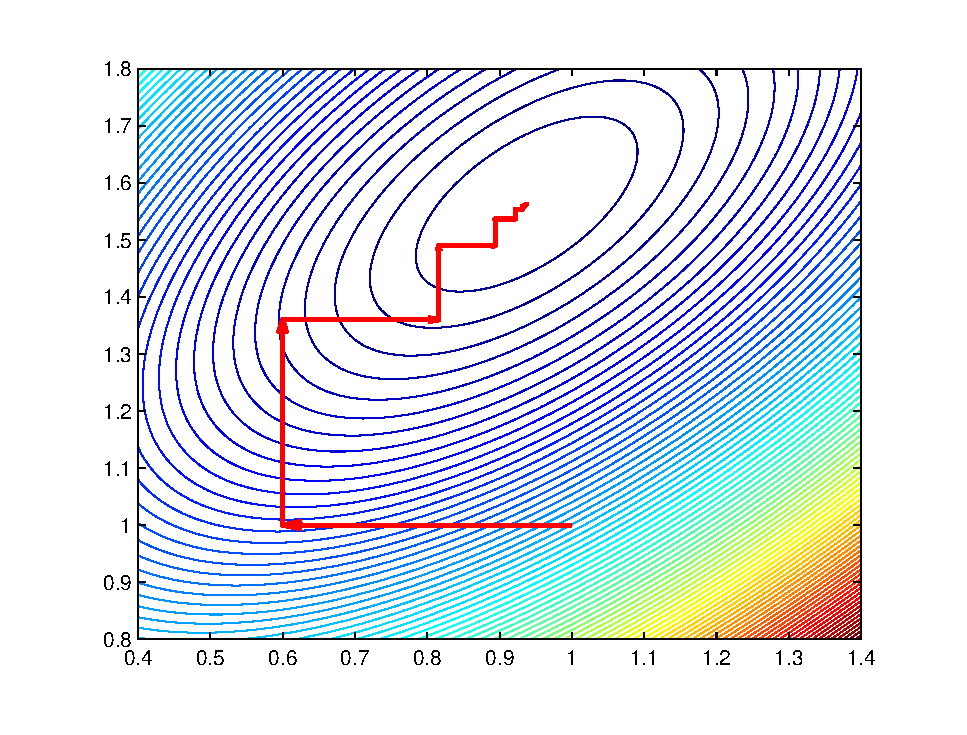
\includegraphics[width=0.45\textwidth]{figure/smooth_coordinate.eps}
    }
    \hfill
	\subfloat[non-smooth objective]{
	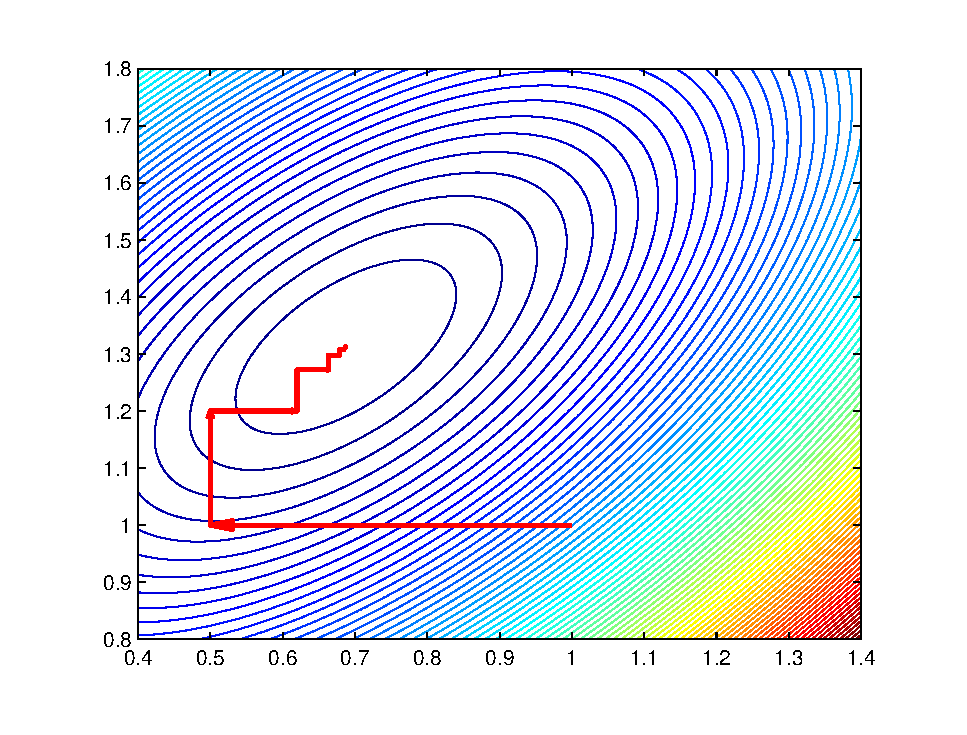
\includegraphics[width=0.45\textwidth]{figure/nonsmooth_coordinate.eps}
    }
\caption{Path of coordinate descent}
\label{fig:scg}
\end{figure}


\subsubsection{LASSO} 
\paragraph{} 
Consider the LASSO problem \eqref{eq:lasso_formulation}, the non-smooth 
part is separable. Minimizing over $\Vx(i)$ with $\Vx(j), j \neq i$ fixed, 
which could obtained by following close solution,
\begin{align*}
	\MA_i^T\MA_i\Vx(i) + \MA_i^T(\MA_{j\neq i}\Vx(j \neq i) - y) + \lambda 
	\partial \abs{\Vx(i)} = 0.
\end{align*}
The solution is given by soft thresholding \eqref{eq:soft_thresholding}, 
\begin{equation*}
	\Vx(i) = S_{\lambda / \MA_i^T \MA_i}
	(\frac{\MA_i^T(y - \MA_{j\neq i}\Vx(j \neq i))}{\MA_i^T \MA_i}). 
\end{equation*}

% \subsection{LARS}

\subsection{SGD}

\subsubsection{Basic Concept}
\paragraph{}
In stochastic gradient descent, the true gradient is approximated by a 
gradient at a single example. The convergence of stochastic gradient descent 
has been analyzed using the theories of convex minimization and of stochastic 
approximation. Briefly, when the learning rates decrease with an appropriate 
rate, and subject to relatively mild assumptions, stochastic gradient descent 
converges almost surely to a global minimum when the objective function is 
convex. SGD could be generalized to SPGD \cite{nitanda2014stochastic} to deal 
with regularized objectives. Recently, SGD with importance sampling 
\cite{zhao2014stochastic} has been developed. 

\paragraph{Numerical Experiments} 



\section{Experiments and Discussion}
Will come soon 






%
%\begin{figure}[tb]
%\centering
%\subfloat[A city market.]{\includegraphics[width=.45\columnwidth]{Lorem}} \quad
%\subfloat[Forest 
%landscape.]{\includegraphics[width=.45\columnwidth]{Ipsum}\label{fig:ipsum}} \\
%\subfloat[Mountain landscape.]{\includegraphics[width=.45\columnwidth]{Dolor}} 
%\quad
%\subfloat[A tile decoration.]{\includegraphics[width=.45\columnwidth]{Sit}}
%\caption[A number of pictures.]{A number of pictures with no common theme.} % 
%The text in the square bracket is the caption for the list of figures while 
%the text in the curly brackets is the figure caption
%\label{fig:esempio}
%\end{figure}
%
















%----------------------------------------------------------------------------------------
%	BIBLIOGRAPHY
%----------------------------------------------------------------------------------------
\newpage
\renewcommand{\refname}{\spacedlowsmallcaps{References}} % For modifying the bibliography heading
\bibliography{reference.bib} % The file containing the bibliography
\bibliographystyle{unsrtnat}

%----------------------------------------------------------------------------------------

\end{document}